\chapter{Introduction} 
Given a starting point $s$, an endpoint $t$ and a set of
polygons $\mathcal{O}$ in the plane, we want to find the shortest path from $s$ to $t$ 
without traveling through the interior of any polygon in $\mathcal{O}$. 
This is an old and well studied problem, and historically there have been two
conceptually different approaches to the problem, one using visibility graphs and
another using the continuous Dijkstra method. 

The visibility graph approach is to construct a graph of all paths between every pair 
of vertices in the plane which doesn't go through an interior of an obstacle. 
These paths are called legal paths. Then the shortest path is found by then running a 
single source shortest path algorithm on that graph. A problem of this approach
is the complexity of the graph can be $\Theta(n^2)$, with $n$ begin the number of vertices of the polygons,
which makes it difficult to get below this threshold. 

The continuous Dijkstra method works by simulating a \emph{wavefront propagation}.
A wavefront is a circular arch which originates from a point and expands in at unit-speed
(non-changing speed) such that all points of the boundary of the arch have equal distance 
$d$ to the generator point from which the wavefront originated, at every time $t$. 
This point is the source (start point) $s$, see figure \ref{fig:simplewavefront}.

\begin{figure}[H]
    \centering
	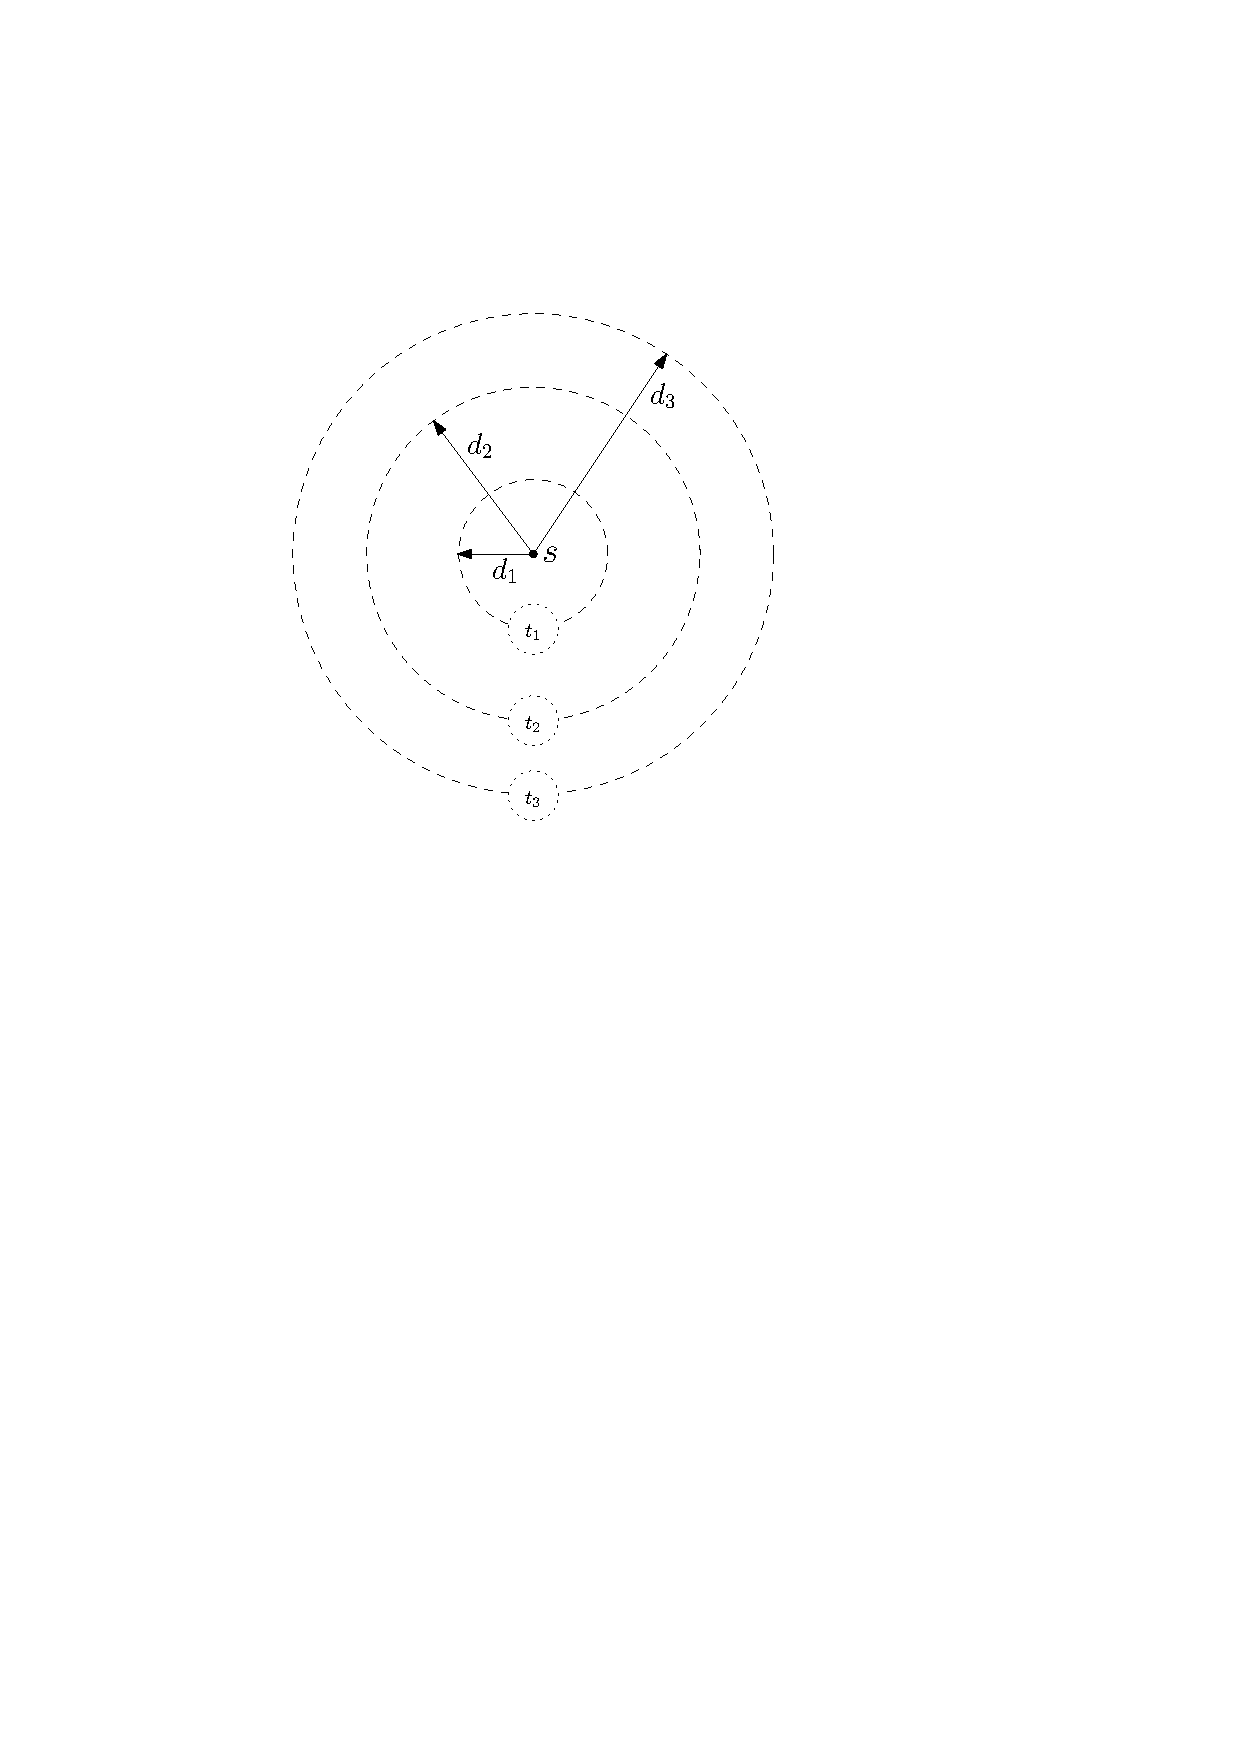
\includegraphics[width=0.5\textwidth]{figures/simplewavefront.pdf}
	\caption{A right turn formed by three points}
    \label{fig:simplewavefront}
\end{figure}

From the figure we can see that since the wavefront expands at unit-speed, the time distance
$d_i$ at time $t_i$ are equal, are one therefore is only concerned with the time $t$.
Every time a vertex $v$ is reached a new wavefront starts emitting from $v$. This way
the plane will be divided into different areas depending on which wavefront encapsulates it,
see figure \ref{fig:introductiontowavefront}.

\begin{figure}[H]
    \centering
	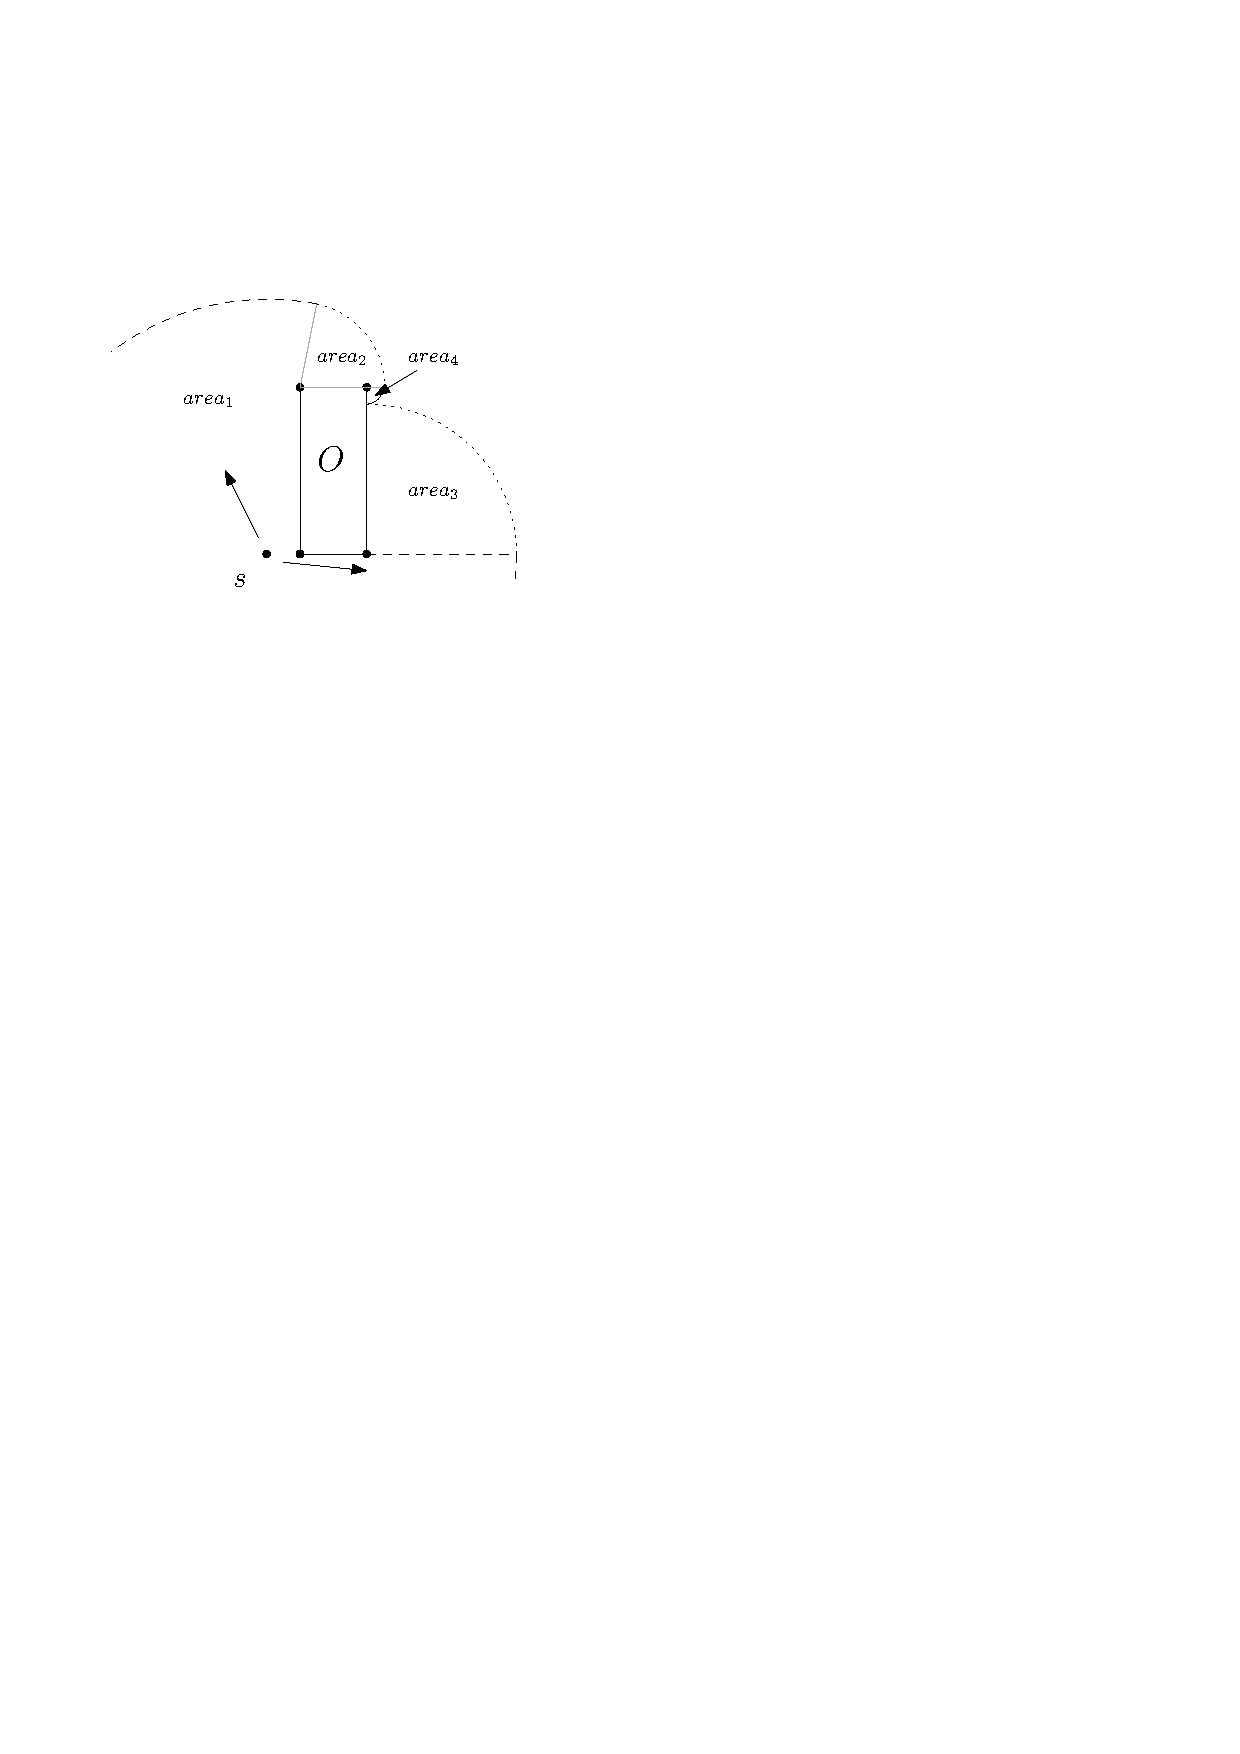
\includegraphics[width=0.5\textwidth]{figures/introductiontowavefront.pdf}
	\caption{A simple example of the wavefront spreading in the plane around an obstacle $O$
	         an encapsulating different areas.}
     \label{fig:introductiontowavefront}
\end{figure}

In 1999 Hershberger and Suri published the paper "an optimal algorithm for euclidean shortest 
paths in the plane"\cite{HershbergerS99} in which they presented an optimal $O(n\log n)$ time 
algorithm which matched the lower bound of the problem (see Chapter \ref{chapter:lowerbound}), 
using an implementation of the continuous Dijkstra method.

In 2017 they, together with Kumar, looked at a generalization of the problem:
given the same setting as before, one is now allowed to go through up to $k$ obstacles.
See figure \ref{fig:shortestkpath}.

\begin{figure}[H]
    \centering
	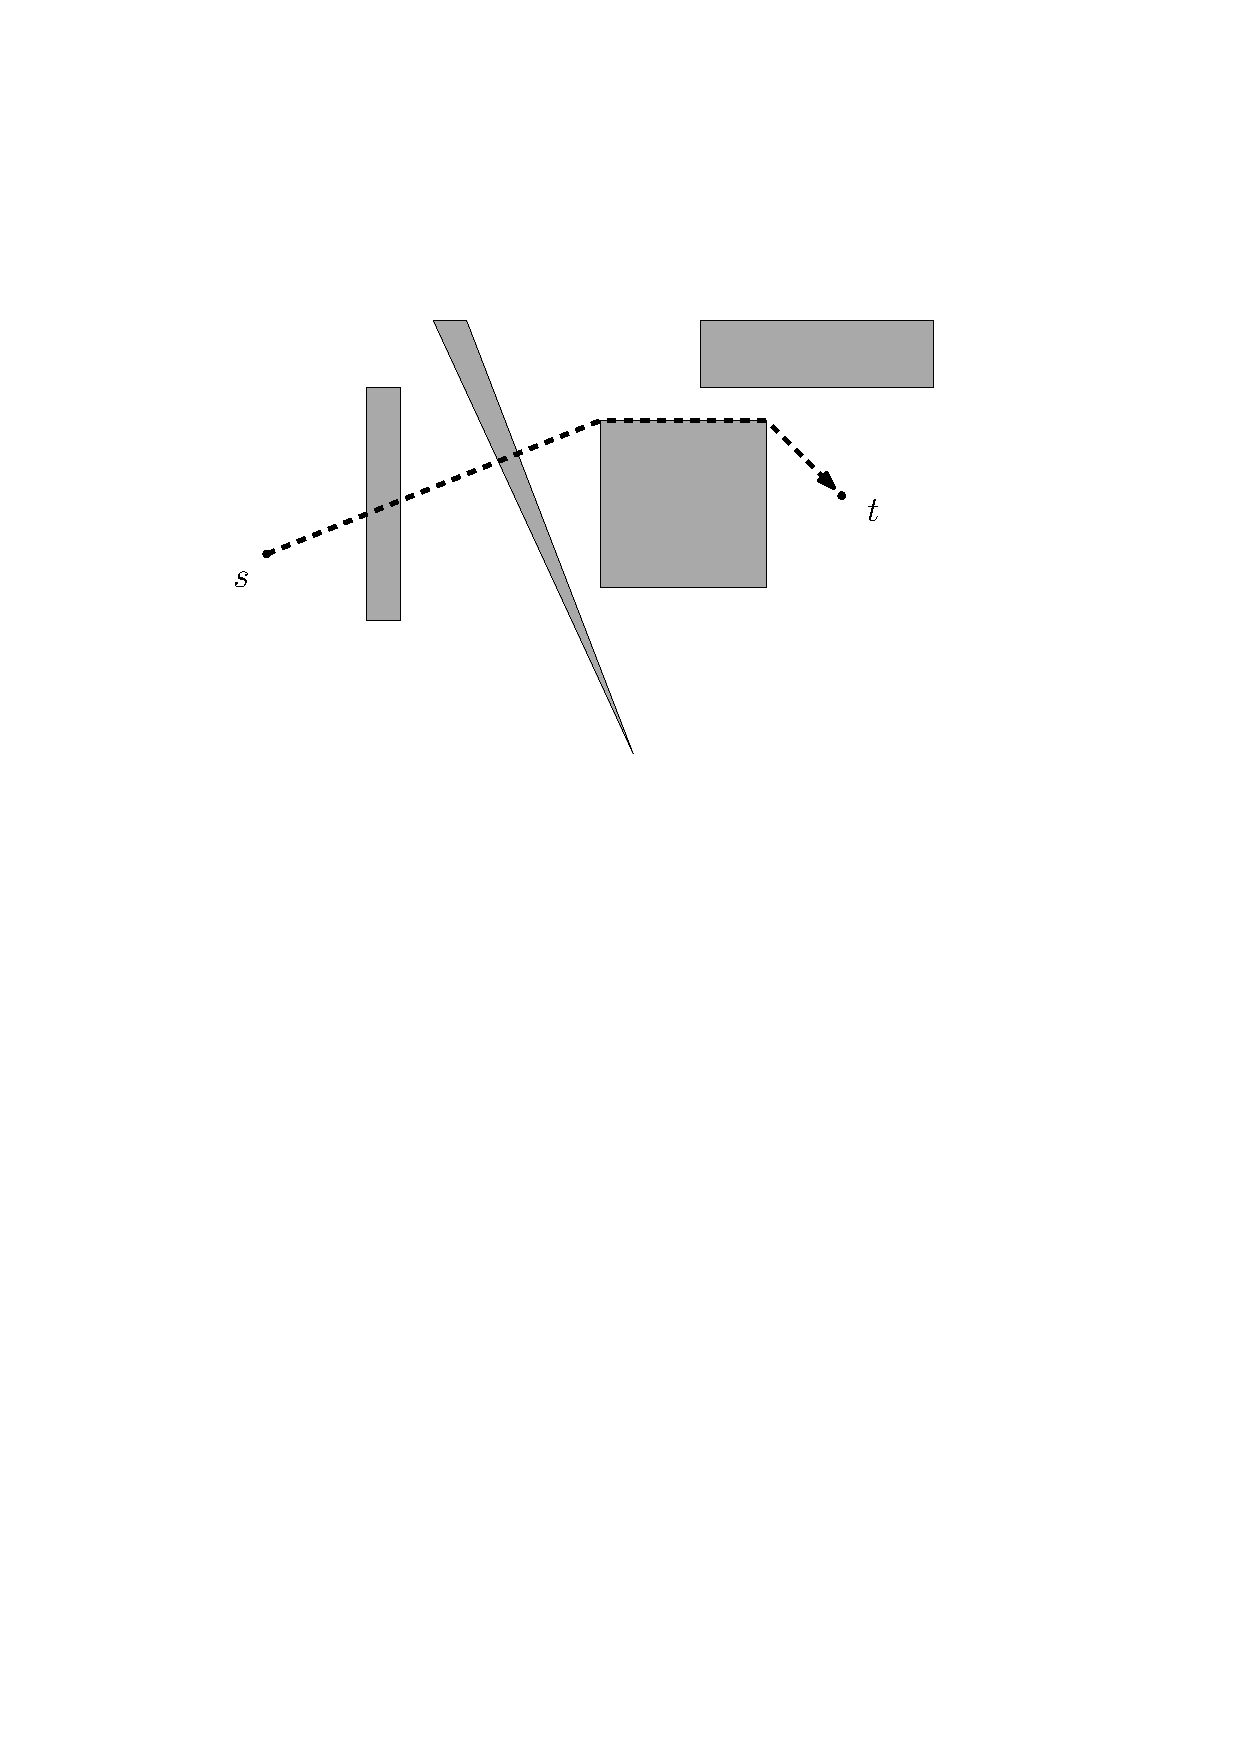
\includegraphics[width=0.7\textwidth]{figures/shortestkpath.pdf}
	\caption{A shortest $k$-path from $s$ to $t$ with $k = 2$}
     \label{fig:shortestkpath}
\end{figure}

The problem lies in which polygons you should pass through to minimize the distance from
$s$ to $t$. They presented an $O(k^2 n\log n)$ algorithm for this problem,
which used a modified version of the 1999 algorithm\cite{HershbergerKS17}.
Notice that if $k = 0$ it is identical to the Shortest path with no violations.

In this thesis we are going to present implementation details of both the original
and the generalized problem. We start by describing and implementing a naive algorithm 
for solving the problem based on computing a visibility graph and then running the Dijkstra
single source shortest path algorithm. Afterwards we are going to explain the theoretical
results leading to the algorithm and the implementation details. Lastly we describe the 
algorithm from 2017 and its implementation details.

\section{Formal Problem description} 
\label{problemdescription}
Given two points in the plane $s,t\in\mathbb{R}^2$ and a list of polygons
$\mathcal{O}=o_1,\dots,o_h$ where $o_i$ is a list of points in polygon $o_i$
starting at an arbitrary place and in clockwise order (note that sometimes we
use $\mathcal{O}$ as a set e.g. polygon $o_i \in \mathcal{O}$). We say a
\emph{legal path} is a list of points where two adjacent points are mutually
visible, i.e. you are able to draw a line from one to the other without
crossing the interior of any polygon in $P$.  We want to find a shortest legal
path from $s$ to $t$.

\section{Previous work}
\begin{table}[H]
\begin{tabular}{ c l l l c c} 
	\hline
	Year & Paper & Run time & Space & Visibility graph & SPM \\
	\hline
	 & Naive\tablefootnote{See Chapter 2} & $O(n^3)$ & $O(|E|)$ & x &\\

	1978 & Lee \cite{LEE78}\tablefootnote{We were not able to obtain the
	original ph.d. thesis, the got the running time from \cite{HershbergerS99} }
	& $O(n^2\log n)$ & ? & x & \\

	1985 & Welzl \cite{DBLP:journals/ipl/Welzl85} & $O(n^2)$ & $O(n^2)$ & x & \\

	1991 & Ghosh et al. \cite{GhoshM91}\tablefootnote{Where $E$ is the number of
	edges in the visibility graph} & $O(E+n\log n)$ & $O(E+n)$ & x & \\

	1991 & Mitchell \cite{DBLP:journals/amai/Mitchell91}\tablefootnote{Where $k$
	is a number bounded by the number of different obstacles that touches any
	shortest path from $s$} & $O(kn \log^2 n)$ & $O(n)$ & & x\\

	1996 & Mitchell \cite{DBLP:journals/ijcga/Mitchell96}\tablefootnote{For any
	$\varepsilon>0$ where the constant in the big-Oh notion depending on
	$\varepsilon$ }& $O(n^{3/2+\varepsilon})$ & $O(n)$ & & x\\

	1999 & Hershberger et al. \cite{HershbergerS99} & $O(n\log n)$ & $O(n\log
	n)$ & & x\\
	\hline
\end{tabular}
\caption{Shortest Paths in the Plane with Polygon obstacles algorithms}
\end{table}

In 1978 Lee presented a $O(n^2\log n)$ algorithm for constructing a visibility
map in his Ph.d.  thesis\cite{LEE78}, we couldn't find the original paper, the
running time is taken from \cite{HershbergerS99}. 

Seven years later, in 1985, Welzl \cite{DBLP:journals/ipl/Welzl85} published a
$O(n^2)$ time algorithm consuming $O(n^2)$ for construction of a visibility
map.  

Six years later in 1991 Ghosh et al.\ \cite{GhoshM91} presented a $O(E+n\log n)$
algorithm consuming $O(E+n)$ space, for constructing a visibility graph where
$E$ is the number of edges in the visibility graph.
Since the visibility graph can contain $O(n^2)$ the algorithm is output bound
and people started making shortest path map algorithm insteed, hoping to reach
the $\Omega{(n\log n)}$ lower bound (see chapter \ref{chapter:lowerbound}).

That same year in 1991 Michell \cite{DBLP:journals/amai/Mitchell91} published
an algorithm for constructing the shortest path map, with running time
$O(kn\log^2 n)$ and $O(n)$ space consumption. Where $k$ is bounded by the
number of different obstacles that touches any shortest path from $s$.

In 1996 he improved the run time to $O(n^{3/2+\varepsilon})$, for any
$\varepsilon>0$ where the constant in big-Oh notion depends on $\varepsilon$
keeping the linear space consumption  \cite{DBLP:journals/ijcga/Mitchell96}.

Then finally in 1999 Hershberger et al.\ \cite{HershbergerS99} revealed a
$O(n\log n)$ algorithm for computing the shortest path map, matching the lower
bound. The space consumption is $O(n\log n)$ and it is still an open problem if
there exists an algorithm with run time $O(n\log n)$ and linear space
consumption.

%\section{Naive algorithm}
%Overview of naive
%\section{Hersberger suri}
%overview of hersberger suri

\section{Overview of thesis}
\begin{description}

	\item[Chapter 2] We descripe a simple $O(n^3)$ algorithm for contructing a
		visibility graph. Then we implement it and compare the run time to the
		theoratical time.

	\item [Chapter 3] Gives an overview of the Hershberger et al.
		\cite{HershbergerS99} algorithm.

	\item [Chapter 4] Goes through the formal definition of the shortest path
		maps and its geometric properties including the complexity of the map.

	\item [Chapter 5] Explaines what the conforming subdivision is and how it is
		contructed.

	\item [Chapter 6] Is dedicated to the wavefront propagation algorithm
		explaining how it works and its implementation details.

	\item [Chapter 7] Presents the Hershberger et al. \cite{HershbergerKS17}
		which shows how to extend the original algorithm to work with $k$
		violations.

	\item [Chapter 8] In here we prove the lower bound of the "shortest path in
		the plane with obstacles problem in The Algebraic Computation Tree Model.
		By making a reduction from number destinction to number sorting to
		shortest map in the plane with obstacles.

	\item [Chapter 9] We conclude the work we have done.

\end{description}
